\documentclass[10pt]{article}
\usepackage[margin=0.72in]{geometry}
\usepackage{amsmath,amssymb,booktabs,graphicx,hyperref}
\title{N16 generic two-torsion action: exact polynomial-ideal certificates}
\author{Frozen 21-model Rosenhain packet}
\date{25 October 2026}
\begin{document}
\maketitle
\noindent The native producer and separate native verifier checked all 105 recorded model/root pairs. On the degree-two locus $U=u(r)\ne0$, all 630 cleared projective cross-products reduce to zero modulo the two Mumford equations. The retained coefficient field, matrices, generators, cross-products, quotient witnesses, and zero remainders are in \texttt{results/generic-ideal.json}. This is a generic-branch certificate, not an all-state law or a new collector measurement.

\begin{center}\begin{tabular}{lr}\toprule Quantity & Verified value\\\midrule
Recorded prime-field models & 21\\
Rational two-torsion roots per model & 5\\
Generic model/root pairs & 105\\
Projective cross-products & 630\\
Nonzero polynomial remainders & 0\\
Quotient-division residual remainders & 0 of 315\\
Clearing denominator & $U^6$ on every pair\\
Maximum sparse cross-product terms & 288\\
Maximum reduction steps per cross-product & 143\\
Exceptional $U=0$ branch theorem & null\\
Degree-one/zero geometric action theorem & null\\
New collector/rho cost ratio & null\\
\bottomrule\end{tabular}\end{center}

\begin{center}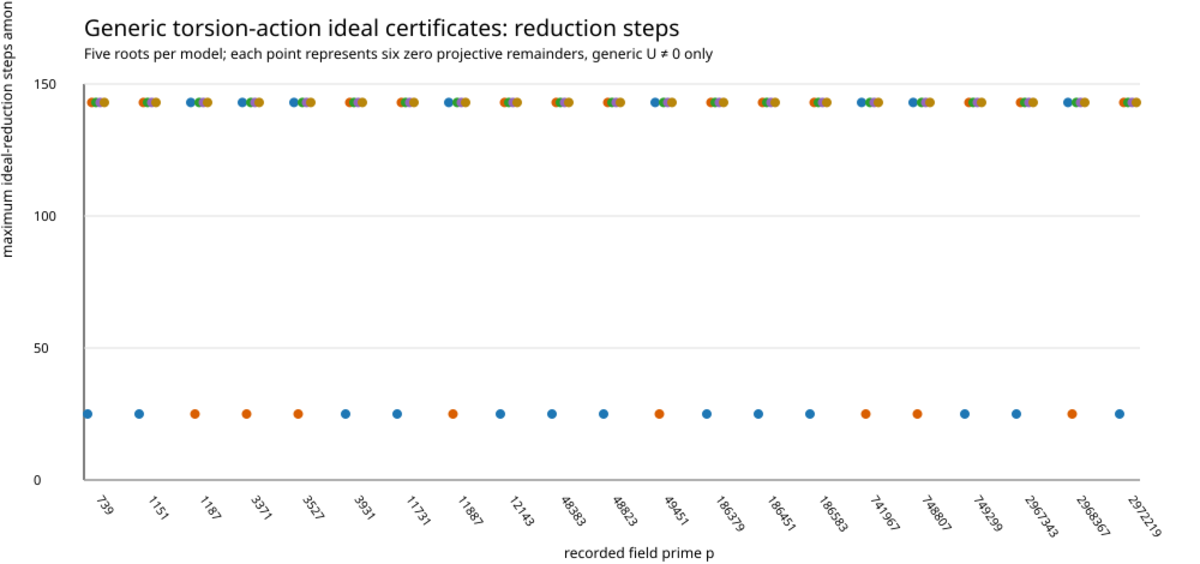
\includegraphics[width=0.94\textwidth]{research/kummer_differential_collector_20261022/n16-action-certificate/generic-ideal-graph.png}\end{center}

\noindent Write $u=x^2+a_1x+a_0$, $v=b_1x+b_0$, and $f\bmod u=R_0+R_1x$. The ideal generators are
\[E_0=b_0^2-a_0b_1^2-R_0,\qquad E_1=2b_0b_1-a_1b_1^2-R_1.\]
For each root $r$, put $U=u(r)$, $V=v(r)$, $L=(Uv-Vu)/U$. Polynomial division of $U^2f-(Uv-Vu)^2$ by $u(x-r)$ yields $q_2x^2+q_1x+q_0$ with $q_2=U^2$ modulo $(E_0,E_1)$. Thus the generic translated divisor has $u'=x^2+(q_1/U^2)x+q_0/U^2$. Its second Mumford coefficient comes from $-L\bmod u'$. The cancelled Kummer chart is converted by the recorded nonsingular matrix $C$; the candidate action matrix is $M_r$.

\noindent The producer clears $U^6$ in the translated four-vector $K'$ and constructs six polynomials $F_{ij}=K'_i(M_rK)_j-K'_j(M_rK)_i$ for $0\le i<j<4$. Every retained certificate explicitly supplies $A_{ij},B_{ij}$ such that $F_{ij}=A_{ij}E_0+B_{ij}E_1$ in $\mathbb F_p[a_0,a_1,b_0,b_1]$. A separate Rust checker reconstructs $f,C_2,M_r$, the translated numerator, all six $F_{ij}$, and these polynomial equalities from the frozen inputs. The degree-two matrix $C_2$ differs from the source degree-one matrix $C_1$; the separate exceptional packet checks both determinants. In all 105 rows, the first transformed coordinate is $W_0=\kappa_r U$ with $\kappa_r\ne0$; hence the projective relation is defined on $U\ne0$.

\noindent The finite exceptional replay in the main N16 report remains separate evidence. This generic certificate by itself does not cover $U=0$ or degree-one/zero classes; the companion exceptional packet checks those identities for the declared charts. Neither packet independently derives the intended geometric Kummer embedding or measures a signed collector with relation-label preservation and cold matched-rho cost. The standardized 105-row CSV, review graph, full raw certificate, exact command, and SHA-256 list accompany this PDF.
\end{document}
